%!TEX root = ../../../_main.tex
\subsection{Twisted weak ordering algorithms}
\label{sec:twisted-involutions-algorithms}

Now we address the problem of calculating $Wk(\theta)$ for an arbitrary Coxeter group $W$, given in form of a set of generating symbols $S = \{s_1, \ldots s_n\}$ and the relations in form of $m_{ij} = \ord(s_i s_j)$. From this input we want to calculate the Hasse diagram, i.e. the vertex set $\ti{\theta}$ and the edges labeled with $\ul s$. Thanks to \ref{lemm:twisted-e-orbit-coincides-with-twisted-involutions} the vertex set can be received by walking the $e$-orbit of the action from \ref{defi:twisted-operation}. The only element of twisted length 0 is $e$. Suppose we have already calculated the Hasse diagram until the twisted length $k$, i.e. we know all vertices $w \in \ti{\theta}$ with $\rho(w) \leq k$ and all edges connecting two vertices $u,v$ with $\rho(u) + 1 = \rho(v) \leq k$. Let $\rho_k := \{ w \in \ti{\theta} : \rho(w) = k \}$. Then all vertices in $\rho_{k+1}$ are of the form $w \ul s$ for some $w \in \rho_k, s \in S$. For each $(w,s) \in \rho_k \times S$, we calculate $w \ul s$. If $\rho(w \ul s) = k + 1$ then $w \prec w \ul s$. To avoid having to check the twisted length we use \ref{lemm:rho-w-ul-s-minus-rho-w-differs-by-1}. We already know the set $S_w \subseteq S$ of all generators yielding an edge into $w$. Due to the lemma it is $\rho(w \ul s) = k - 1$ for all $s \in S_w$ and $\rho(w \ul s) = k + 1$ for all $s \in S \setminus S_w$. Hence we only calculate $w \ul s$ for $s \in S \setminus S_w$ and know $w \prec w \ul s$ without checking the twisted length explicitly. The last problem to solve is the possibility of two different $(w,s),(v,t) \in \rho_k \times S$ with $w \ul s = v \ul t$. To deal with this, we have to compare a potential new twisted involution $w \ul s$ with each element of twisted length $k+1$, already calculated. The concrete problem of comparing two elements in a free presented group, called \defword{wordproblem for groups}, will not be addressed here. We suppose, that whatever computer system is used to implement our algorithm, supplies a suitable way to do that. The only thing to note is, that solving the wordproblem is not a cheap operation. Reducing the count of element comparisions is a major demand to any algorithm, calculating $Wk(\theta)$.

The steps discussed have been compiled in to an algorithm by Haas \cite[Algorithm 3.1.1]{haas:twoa}. We take this as our starting point. Since the runtime is far from being optimal, we use the structural properties of rank-2-residuums from Section \ref{sec:twisted-involutions-residuums} to improve the algorithm. As we will show, these optimizations yield an algorithm with an asymptotical perfect runtime behavior. \ref{algo:twoa1} shows the algorithm of Haas.

\begin{algo}[TWOA1]
	\hfill
	\namedlabel{algo:twoa1}
	\begin{algorithmic}[1]
	\Procedure{TwistedWeakOrderingAlgorithm1}{$(W,S),k_{max}$} 
	\State $V \gets \{(e,0)\}$
	\State $E \gets \{\}$

	\For{$k \gets 0 \textbf{ to } k_{max}$} \label{algo:twoa1-k-loop}
		\ForAll{$(w,k_w) \in V \textbf{ with } k_w = k$} \label{algo:twoa1-v-loop}
			\ForAll{$s \in S \textbf{ with } \nexists (\cdot,w,s) \in E$} \label{algo:twoa1-s-loop} \Comment{Only for $s \notin D_R(w)$}
				\State $y \gets ws$
				\State $z \gets \theta(s)y$
				\If{$z=w$} \label{algo:twoa1-check-one-or-bothsided}
					\State $x \gets y$
					\State $t \gets s$
				\Else
					\State $x \gets z$
					\State $t \gets \ul s$
				\EndIf
				
				\State $isNew \gets \textbf{true}$
				\ForAll{$(w',k_{w'}) \in V \textbf{ with } k_{w'} = k+1$} \label{algo:twoa1-comp} \Comment{Check if $x$ already known}
					\If{$x = w'$}
						\State $isNew \gets \textbf{false}$
					\EndIf
				\EndFor
				
				\If{$isNew = \textbf{true}$}
					\State $V \gets V \cup \{ (x,k+1) \}$
				\EndIf
				\State $E \gets E \cup \{ (w,x,t) \}$
			\EndFor
		\EndFor
		\State $k \gets k + 1$
	\EndFor

	\State \textbf{return} $(V,E)$\Comment{The poset graph}
	\EndProcedure
	\end{algorithmic}
\end{algo}

Note, that if $W$ is finite, $k_{max}$ does not have to be evaluated explicitly. When $k$ reaches the maximal twisted length in $Wk(\theta)$, then the only vertex of twisted length $k$ is the unique element $w_0 \in W$ of maximal ordinary length. Since $s \in D_R(w_0)$ for all $s \in S$, there is no $s' \in S$ remaining to calculate $w_0 \ul s'$ for. This condition can be checked to terminate the algorithm without knowing $k_{max}$ before. When $W$ is infinite, there is no maximal element and $\ti{\theta}$ is infinite, too. In this case $k_{max}$ is used to terminate after having calculated a finite part of $Wk(\theta)$.

\begin{lemm}
	\ref{algo:twoa1} is a deterministic algorithm.

	\begin{proof}
		The outer loop (line \ref{algo:twoa1-k-loop}) is strictly ascending in $k \in \{0,\ldots,k_{max}\}$ and so finite. The innermost loop (line \ref{algo:twoa1-s-loop}) is finite since $S$ is finite. The inner loop (line \ref{algo:twoa1-v-loop}) is finite, since $V$ starts as finite set and in each step there are added at most $|V| \cdot |S|$ many new vertices. Therefore the algorithm terminates. The soundness is due to the arguments at the beginning of Section \ref{sec:twisted-involutions-algorithms}.
	\end{proof}
\end{lemm}

\begin{lemm}
	Let $k \in \nn$, $n = |\{ w \in \ti{\theta} : \rho(w) \leq k \}|$ and for $0 \leq i \leq k$ let $\rho_i = |\{ w \in \ti{\theta} : \rho(w) = i \}|$. Then $\ref{algo:twoa1} \in \mathcal{O}(n^2/k)$.

	\begin{proof}
		Our algorithm has to do at least $\rho_i (\rho_i - 1)/2$ many element comparisons (line \ref{algo:twoa1-comp}) for each $0 \leq i \leq k$. Set $m = \lfloor \frac{n}{k} \rfloor$. In the most optimistic case it is $\rho_i \geq m$ for all $i$. In practice the situation will be worse, since some $\rho_i$ will be smaller than $m$ (for example $\rho_0 = 1$) and so some $\rho_i$ will be much larger than $m$. This optimistic case yields at least $m(m-1)/2 \cdot k$ many element comparisons. Hence regarding the most delimiting operation, the element comparison, our algorithm is in $\Omega(m^2k) = \Omega(n^2 / k)$. The element comparison at line \ref{algo:twoa1-check-one-or-bothsided} done at most $n \cdot |S|$. Other operations, like for example insertion into or searching in sets can be considered super linear, if for example sets are ordered immediately at insertion and then searching is done with binary search. So the algorithm is in $\mathcal{O}(n^2 / k)$.
	\end{proof}
\end{lemm}

\begin{coro}
	Let $k \in \nn$ and $n = |\{ w \in \ti{\theta} : \rho(w) \leq k \}|$. Then any algorithm calculating $Wk(\theta)$ is in $\Omega(n)$.

	\begin{proof}
		Any algorithm must at least return $\{ w \in \ti{\theta} : \rho(w) \leq k \}$ and this set is of size $n$.
	\end{proof}
\end{coro}

Our goal is to improve \ref{algo:twoa1} so that we get an algorithm in $\mathcal{O}(n)$, i.e. an asymptotical perfect algorithm for calculating $Wk(\theta)$. As already seen the element comparison of a potential new element with all already known elements of same twisted length (line \ref{algo:twoa1-comp}) is the bottleneck. Here the rank-2-residuums become key. Suppose we have a $w \in \ti{\theta}$ with $\rho(w) = k$ and $s \in S$. In \ref{algo:twoa1} we would now check, if $w \ul s$ is a new vertex, or if we already calculated it by comparing it with all already known vertices of twisted length $k + 1$. Assume it is already known. This means there is another twisted involution $v$ with $\rho(v) = k$ and another generator $t \in S$ with $v \ul t = w \ul s$. With \ref{prop:rank-2-residuums-are-convex} $w \ul s$ is the unique element of maximal twisted length in the rank-2-residuum $wC_{\{s,t\}}$. This yields a necessary condition for $w \ul s$ to be equal to a already known vertex, allowing us to replace the ineffective search all method in \ref{algo:twoa1}, line \ref{algo:twoa1-comp}.

\begin{figure}[ht]
	\centering
	%!TEX root = ../../_main.tex
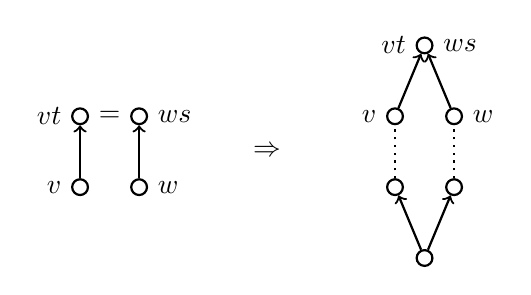
\begin{tikzpicture}[scale=1,bend angle=10]
\newcommand{\xspace}{1}
\newcommand{\yspace}{0.6}
\tikzstyle{vertex}=[draw,thick,circle,minimum size=2mm,inner sep=1pt]
\tikzstyle{edge}=[thick,->]
\tikzstyle{edge2}=[dotted,thick]
\tikzstyle{onesided}=[edge,dashed]
\tikzstyle{bothsided}=[edge]

\node[vertex, label=180:$v$] (3) at (\xspace*-0.375,\yspace*1.5) {};
\node[vertex, label=360:$w$] (4) at (\xspace*0.375,\yspace*1.5) {};
\node[vertex, label=180:$v \ul t$] (5) at (\xspace*-0.375,\yspace*3.0) {};
\node[vertex, label=360:$w \ul s$] (6) at (\xspace*0.375,\yspace*3.0) {};
\node (7) at (\xspace*0,\yspace*3.0) {$=$};
\draw[bothsided] (3) edge (5);
\draw[bothsided] (4) edge (6);

\node (then) at (\xspace*2,\yspace*2.25) {$\Rightarrow$};

\node[vertex] (0) at (4+\xspace*0,\yspace*0) {};
\node[vertex] (1) at (4+\xspace*-0.375,\yspace*1.5) {};
\node[vertex] (2) at (4+\xspace*0.375,\yspace*1.5) {};
\node[vertex, label=180:$v$] (3) at (4+\xspace*-0.375,\yspace*3.0) {};
\node[vertex, label=360:$w$] (4) at (4+\xspace*0.375,\yspace*3.0) {};
\node[vertex, label=180:$v \ul t$, label=360:$w \ul s$] (5) at (4+\xspace*0,\yspace*4.5) {};
\draw[bothsided] (0) edge (1);
\draw[bothsided] (0) edge (2);
\draw[edge2] (1) edge (3);
\draw[edge2] (2) edge (4);
\draw[bothsided] (3) edge (5);
\draw[bothsided] (4) edge (5);
\end{tikzpicture}
	\caption{Optimization of \ref{algo:twoa1}}
	\label{fig:optimization-of-twoa1}
\end{figure}

\begin{lemm}
	\typedlabel{lemm:twoa1-necessary-condition-for-ws-eq-vt}
	Let $k \in \nn$ and suppose we are in the sitation described at the beginning of Section \ref{sec:twisted-involutions-algorithms}. Let $\rho_i := \{ w \in \ti{\theta} : \rho(w) = i \}$ and $\rho'_{k+1}$ the set of the already calculated vertices with twisted length $k+1$. If $w \ul s \in \rho'_{k+1}$ for some $w \in \rho_k, s \in S$, say $w \ul s = v \ul t$ with $v \in \rho_k$ and $t \in S \setminus \{s\}$, then $w \ul s = w[\ul t \ul s]^n$ for some $n \in \nn$ with $w[\ul t \ul s]^j \in \rho_0 \cup \ldots \cup \rho_k \cup \rho'_{k+1}$ for $1 \leq j \leq n$.

	\begin{proof}
		The equality $w \ul s = w[\ul t \ul s]^n$ for some $n \in \nn$ is due to \ref{prop:rank-2-residuums-are-convex}. All vertices in this rank-2-residuum except $v \ul t$ have a twisted length of $k$ or lower. For $v \ul t$ we supposed it is already known, hence $v \ul t \in \rho'_{k+1}$. Therefore all vertices $w[\ul t \ul s]^j$, $1 \leq j \leq n$ are in $\rho_0 \cup \ldots \cup \rho_k \cup \rho'_{k+1}$.
	\end{proof}
\end{lemm}

This can be checked effectively. Both, $w$ and $s$ are fixed. Start with $M = \emptyset$. For all already known edges from or to $w$ being labeled with $\ul t \in \ul S \setminus \{\ul s\}$ we do the following: Walk $w[\ul t \ul s]^i$ for $i = 0,1,\ldots$ until $\rho(w[\ul t \ul s]^i) = k + 1$. Note that walking in this case really means walking the graph. All involved vertices and edges have already been calculated. So there is no need for more calculations in $W$ to find $w[\ul t \ul s]^i$. By \ref{prop:rank-2-residuums-are-convex} such a path must exist (in a completely calculated graph). But we could be in the case, where the last step from $w[\ul t \ul s]^{i-1}$ to $w[\ul t \ul s]^{i}$ has not been calculated yet. If it is already calculated, then add this element to $M$ by setting $M = M \cup \{ w[\ul t \ul s]^{i} \}$. If not, do not add it to $M$.

Now $M$ contains all already known elements of twisted length $k+1$, satisfying the necessary condition from \ref{lemm:twoa1-necessary-condition-for-ws-eq-vt}. Furthermore $|M| < |S|$. So for each pair $(w,s)$ we have to do at most $|S|-1$ many element comparisons the determine, if $w \ul s$ is new or already known, no matter how many elements of twisted length $k+1$ are already known. We can get even more information from the rank-2-residuums:

\begin{lemm}
	Let $w \in \ti{\theta}$ with $\rho(w) = k$, $s,t$ be two distinct generators and $s \notin D_R(w)$. Suppose $n \in \nn$ to be the smallest number for that $\rho(w[\ul t \ul s]^{2n-1}) = k + 1$ holds. Then:

	\begin{enumerate}
		\item If $n = \ord(st)$, then $w[\ul t \ul s]^{2n-1} = w \ul s$.
		\item If $n \geq 2$ and $l(w[\ul t \ul s]^{2n-1}) - l(w[\ul t \ul s]^{2n-2}) = 1$, then $w[\ul t \ul s]^{2n-1} = w \ul s$.
	\end{enumerate}

	\begin{proof}

		\begin{enumerate}
			\item Follows immediately from \ref{lemm:max-twisted-circle-height}.
			\item Because of the length difference the step from $w[\ul t \ul s]^{2n-2}$ to $w[\ul t \ul s]^{2n-1}$ is a multiplication, not a twisted conjugation, and because of $n \geq 1$ this step cannot be next to the smallest element in $wC_{\{s,t\}}$. Hence $w[\ul t \ul s]^{2n-1} = w \ul s$ by \ref{coro:onesided-operations-only-at-top-or-bottom-end-of-twocycle}. \qedhere
		\end{enumerate}
	\end{proof}
\end{lemm}

\begin{lemm}
	Let $w \in \ti{\theta}$ with $\rho(w) = k$, $s,t$ be two distinct generators and $s \notin D_R(w)$. Suppose $w[\ul t \ul s]^{2n-1} = w \ul s$ and suppose $n$ to be the smallest number with this property. Then $w[\ul t \ul s]^{n-1}$ is the minimal element $\min(w,\{s,t\})$ and $w[\ul t \ul s]^{2n-1}$ is the maximal element. Define
	\begin{align*}
		a & = l(w \ul s) - l(w), \\
		b & = l(w[\ul t \ul s]^{n-1}) - l(w[\ul t \ul s]^{n-2}), \\
		c & = l(w[\ul t \ul s]^{n}) - l(w[\ul t \ul s]^{n-1}) \textrm{ and} \\
		d & = l(w[\ul t \ul s]^{2n-1}) - l(w[\ul t \ul s]^{2n-2}).
	\end{align*}
	Note that $a,b,c,d \in \{1,2\}$ contain the information, if edges next to the minimal and the maximal element of $wC_{\{s,t\}}$ are twisted conjugations or multiplications. Then each can be deduced from the three remaining ones with the equation $(a+b+c+d) \equiv 0 \mod 2 $.

	\begin{proof}
		The minimality of $w[\ul t \ul s]^{n-1}$ and the maximality of $w[\ul t \ul s]^{2n-1}$ is due to \ref{prop:rank-2-residuums-are-convex}. The soundness of the equation follows from the symmetric distribution of twisted conjugations and mutipliations from \ref{lemm:one-both-sided-action-symmetric-in-rank-2-residuums}.
	\end{proof}
\end{lemm}

\begin{algo}[TWOA2]
	\hfill
	\namedlabel{algo:twoa2}
	\begin{algorithmic}[1]
	\Procedure{TwistedWeakOrderingAlgorithm1}{$(W,S),k_{max}$} 
	\State $V \gets \{(e,0)\}$
	\State $E \gets \{\}$

	\For{$k \gets 0 \textbf{ to } k_{max}$} \label{algo:twoa2-k-loop}
		\ForAll{$(w,k_w) \in V \textbf{ with } k_w = k$} \label{algo:twoa2-v-loop}
			\ForAll{$s \in S \textbf{ with } \nexists (\cdot,w,s) \in E$} \label{algo:twoa2-s-loop} \Comment{Only for $s \notin D_R(w)$} \Comment{\todo}
			\EndFor
		\EndFor
		\State $k \gets k + 1$
	\EndFor

	\State \textbf{return} $(V,E)$\Comment{The poset graph}
	\EndProcedure
	\end{algorithmic}
\end{algo}

\newpage

\begin{table}
	\centering
	\begin{tabular}{|c|c|c|r|r|r|r|}
	\hline
	\multicolumn{3}{|c|}{} & \multicolumn{2}{c|}{Timings} & \multicolumn{2}{c|}{Element comparisons}\\
	\hline
	$W$ & $|Wk(W,\id)|$ & $\rho(w_0)$ & \ref{algo:twoa1} & \ref{algo:twoa2} & \ref{algo:twoa1} & \ref{algo:twoa2}\\
	\hline
	$A_9$ & 9496 & 25 & 00:02.180 & 00:01.372 & 13,531,414 & 42,156\\
	\hline
	$A_{10}$ & 35696 & 30 & 00:31.442 & 00:06.276 & 185,791,174 & 173,356\\
	\hline
	$A_{11}$ & 140152 & 36 & 11:04.241 & 00:29.830 & 2,778,111,763 & 737,313\\
	\hline
	$E_6$ & 892 & 20 & 00:03.044 & 00:00.268 & 85,857 & 2,347\\
	\hline
	$E_7$ & 10208 & 35 & 06:11.728 & 00:02.840 & 7,785,186 & 29,687\\
	\hline
	$E_8$ & 199952 & 64 & -- & 11:03.278 & -- & 682,227\\
	\hline
	\end{tabular}
	\caption{Benchmark}
	\label{tab:benchmark-twoa}
\end{table}